\documentclass[tikz,border=10pt]{standalone}
\usepackage[T1]{fontenc}
\usepackage{helvet}
\renewcommand{\familydefault}{\sfdefault}
\usepackage{tikz}
\usetikzlibrary{arrows.meta,positioning,shapes.multipart,shapes.geometric,fit,backgrounds,calc,shadows}

\definecolor{navy}{HTML}{1F3A5F}
\definecolor{teal}{HTML}{0C6B58}
\definecolor{amber}{HTML}{D9822B}
\definecolor{crimson}{HTML}{B42318}
\definecolor{violet}{HTML}{6B21A8}
\definecolor{sky}{HTML}{2186EB}
\definecolor{slate}{HTML}{486581}
\definecolor{mist}{HTML}{F0F4F8}
\definecolor{line}{HTML}{9FB3C8}

\tikzset{
  >={Stealth[length=2.6mm]},
  box/.style={draw=navy, very thick, rounded corners=3pt, fill=white, align=center,
    inner sep=5pt, font=\small, minimum height=9mm},
  softbox/.style={box, draw=slate, thick, fill=mist},
  layer/.style={draw=line, dashed, rounded corners=6pt, inner sep=7pt},
  layertitle/.style={font=\bfseries\small, text=slate, anchor=north west},
  flow/.style={->, thick, draw=navy},
  dflow/.style={->, thick, draw=slate, dashed},
  lbl/.style={font=\scriptsize, text=slate, fill=white, inner sep=1.5pt},
  umlclass/.style={draw=navy, thick, fill=white, rectangle split, rectangle split parts=3,
    rectangle split part fill={navy!12,white,white}, align=left, font=\scriptsize,
    inner sep=3pt, text width=#1},
  umlclass/.default=38mm,
}

\tikzset{
  term/.style={box, rounded corners=10pt, draw=teal, minimum width=3.6cm, font=\small},
  proc/.style={box, minimum width=5.6cm, font=\small},
  dec/.style={diamond, aspect=2.4, draw=amber, very thick, fill=white, align=center,
    font=\small, inner sep=1pt},
}
\begin{document}
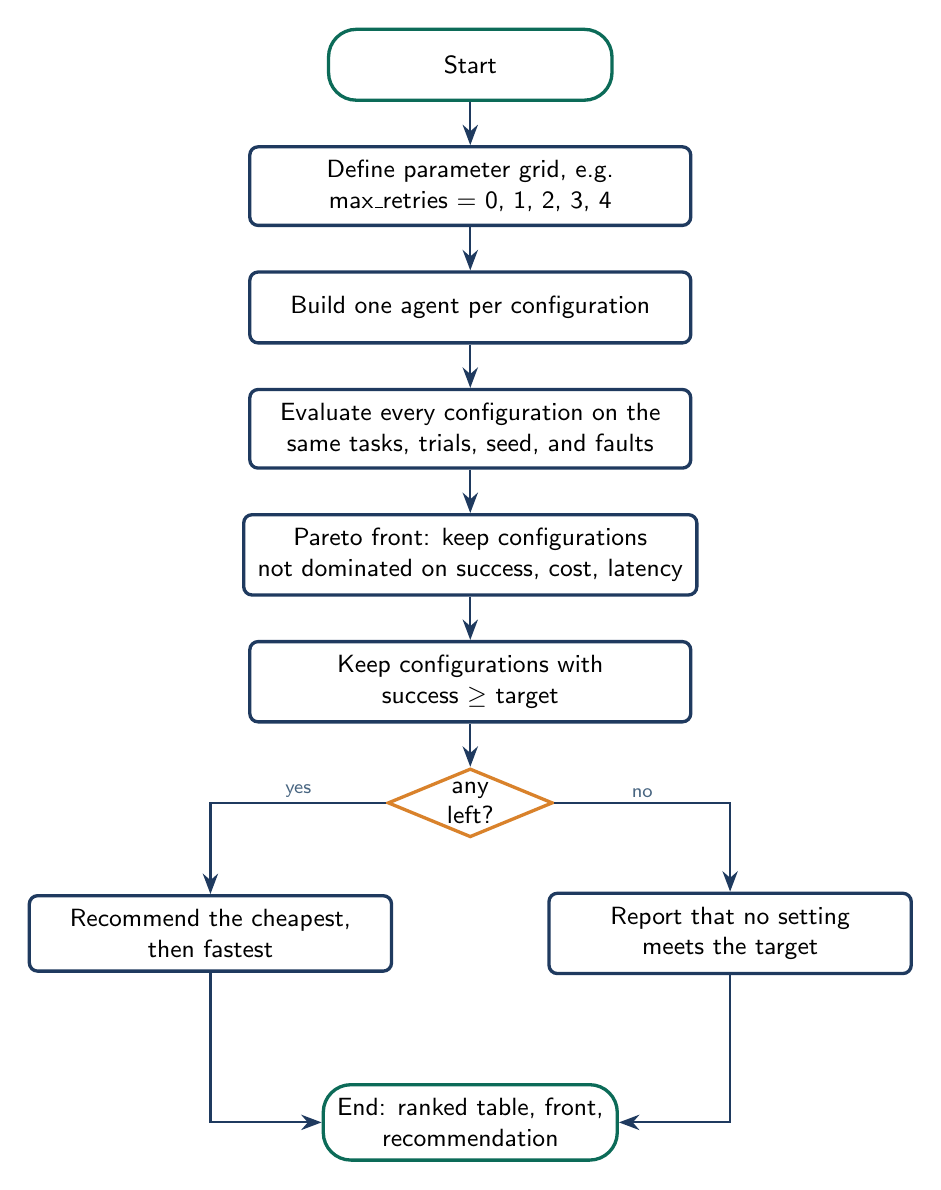
\begin{tikzpicture}[x=1cm,y=1cm, node distance=0.55cm]
  \node[term] (start) {Start};
  \node[proc, below=of start] (grid) {Define parameter grid, e.g.\\ max\_retries = 0, 1, 2, 3, 4};
  \node[proc, below=of grid] (cfg) {Build one agent per configuration};
  \node[proc, below=of cfg] (eval) {Evaluate every configuration on the\\ same tasks, trials, seed, and faults};
  \node[proc, below=of eval] (front) {Pareto front: keep configurations\\ not dominated on success, cost, latency};
  \node[proc, below=of front] (filter) {Keep configurations with\\ success $\ge$ target};
  \node[dec, below=of filter] (any) {any\\ left?};
  \node[proc, minimum width=4.6cm] (pick) at ($(any.south)+(-3.3,-1.2)$) {Recommend the cheapest,\\ then fastest};
  \node[proc, minimum width=4.6cm] (none) at ($(any.south)+(3.3,-1.2)$) {Report that no setting\\ meets the target};
  \node[term, below=3.1cm of any] (stop) {End: ranked table, front,\\ recommendation};

  \draw[flow] (start) -- (grid);
  \draw[flow] (grid) -- (cfg);
  \draw[flow] (cfg) -- (eval);
  \draw[flow] (eval) -- (front);
  \draw[flow] (front) -- (filter);
  \draw[flow] (filter) -- (any);
  \draw[flow] (any.west) -| node[lbl, above, pos=0.25] {yes} (pick.north);
  \draw[flow] (any.east) -| node[lbl, above, pos=0.25] {no} (none.north);
  \draw[flow] (pick.south) |- (stop.west);
  \draw[flow] (none.south) |- (stop.east);
\end{tikzpicture}
\end{document}
